\subsection{Schwingungen}
\subsubsection{Freie Schwingung}
\bsp{Beispiel}

\begin{minipage}{0.47\textwidth}
    Feder~-~Dämpfer~-~System.
    
    Eine Masse $m$ hängt an einer Feder und ist
    an einen Flüssig-Dämpfer angeschlossen.
\end{minipage}
\begin{minipage}[r]{0.49\textwidth}
    \hfill
    \begin{circuitikz}
        \draw (-1,0) -- (1,0);
        \foreach \x in {-9,...,9}
            \draw ( {(\x-1)/10}, 0.1 ) -- ({\x/10},0);
        \coordinate (mass) at (0,-1.7);
        \draw (0,0) to [L] (mass) ;
        \node at (0,-1) [right,xshift=0.2cm] {Federkonstante $k$} ;
        \fill (mass) circle [radius=0.2] node[left,xshift=-0.1cm] {$m$};
        \draw (mass) -- (0,-3) -- + (0.5,0) -- + (-0.5,0);
        \draw (-1,-2.5) -- ++ (0,-1) -- ++ (2,0) -- ++ (0,1);
        \draw[decorate,decoration=snake] (-1, -2.7) -- ++ (2,0);
        \node[right] at (1,-3) {Dämpfer $r$};
        \draw[->] (-1.5,-3) -- ++ (0,2.5) node[midway,left] {$x$};
    \end{circuitikz}
\end{minipage}

DGL: $F=a m = -k x-r \dot{x}$
\begin{equation*}
\boxed{\ddot{x} + \frac{r}{m}\dot{x}+\frac{k}{m} x=0}
\end{equation*}
Freie, gedämpfte Schwingung

Lösung:
\begin{equation*}
    \ddot{x} + \underbrace{\frac{r}{m}}_{2\delta}\dot{x}+
    \underbrace{\frac{k}{m}}_{\omega_0^2} x=0
\end{equation*}
\begin{eqnarr}
    \delta^2 - \omega_0^2 &=&  \left( \frac{r}{2m} \right)^2-\frac{k}{m}\\
    &>& 0 \Rightarrow \text{Fall 1 (Kriechfall)} \\
    &=& 0 \Rightarrow \text{Fall 2 (aperiodischer Grenzfall)} \\
    &<& 0 \Rightarrow \text{Fall 3 (Schwingungsfall)} \\
\end{eqnarr}

\underline{a) Starke Dämpfung (Kriechfall)}
\begin{equation*}
    \boxed{\delta>\omega_0}
\end{equation*}
\begin{equation*}
    \lambda_{1,2} = -\delta\pm\underbrace{\sqrt{\delta^2-\omega_0^2}}_
    {>0 \text{ und }<\delta}<0
\end{equation*}
Lösung: \begin{equation*}
    x(t) = C_1 e^{\lambda_1 t} + C_2 e^{\lambda_2 t}
\end{equation*}
\begin{center}
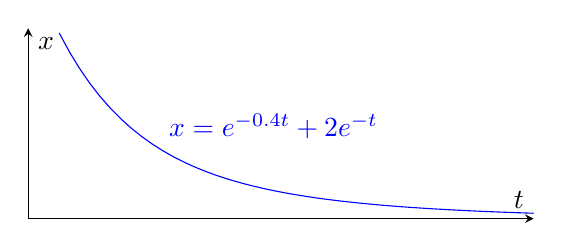
\begin{tikzpicture}
\begin{axis}[
        width = 8cm,
        height = 4cm,
        axis lines = middle,
        clip = false,
        xmin = 0,
        ymin = 0,
        ymax = 2.2, 
        restrict y to domain=0:2.2,
        ticks=none,
        xlabel = $t$,
        ylabel = $x$,
    ]

    \addplot+[mark=none,samples=50,unbounded coords=jump,domain=0:7 ]
    {1*exp(-0.4*x)+2*exp(-x)}
    [yshift=8pt] node [pos=0.27,right] { $x=e^{-0.4t}+2e^{-t} $ } ;
\end{axis}
\end{tikzpicture}
\end{center}

\underline{b) Aperiodischer Grenzfall}
\begin{equation*}
    \boxed{\delta=\omega_0}
\end{equation*}
\begin{equation*}
    \lambda = -\delta
\end{equation*}
Lösung: \begin{equation*}
    x(t) = C_1 e^{-\delta t} + C_2 t e^{-\delta t}
\end{equation*}
\begin{center}
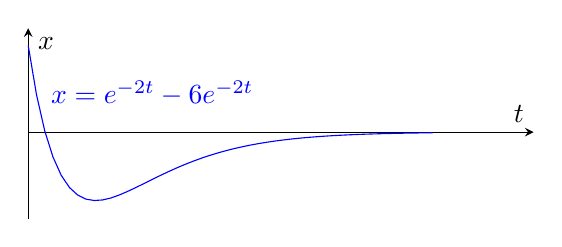
\begin{tikzpicture}
\begin{axis}[
        width = 8cm,
        height = 4cm,
        axis lines = middle,
        clip = false,
        xmin = 0,
        xmax = 5,
        ymin = -1,
        ymax = 1.2, 
        restrict y to domain=-1:2,
        ticks=none,
        xlabel = $t$,
        ylabel = $x$,
    ]

    \addplot+[mark=none,samples=50,unbounded coords=jump,domain=0:4 ]
    {1*exp(-2*x)-6*x*exp(-2*x)}
    [yshift=8pt] node [pos=0.15,right] { $x=e^{-2t}-6e^{-2t} $ } ;
\end{axis}
\end{tikzpicture}
\end{center}

\underline{c) Schwache Dämpfung}
\begin{equation*}
    \boxed{\delta<\omega_0}
\end{equation*}
\begin{equation*}
    \omega_d = \sqrt{\omega_0^2-\delta^2}<\omega_0
\end{equation*}
Lösung: \begin{eqnarr}
    x(t)&=&  e^{-\delta  t} \left[
        C_1\sin(\omega_d  t) +
        C_2\cos(\omega_d  t) 
        \right]\\
        &=& C e^{-\delta  t} 
        \sin\left( \omega_d t+\phi_d \right)\\
        &=& C e^{-\delta  t} 
        \cos\left( \omega_d t+\varphi_d \right)
\end{eqnarr}

\begin{center}
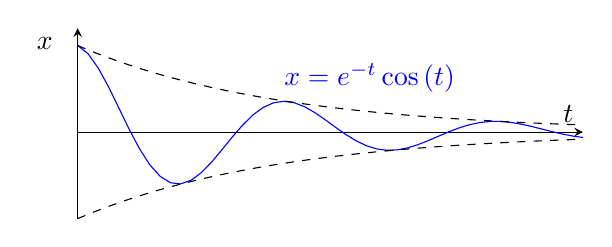
\begin{tikzpicture}
\begin{axis}[
        width = 8cm,
        height = 4cm,
        axis lines = middle,
        clip = false,
        xmin = 0,
        xmax = 5,
        ymin = -1,
        ymax = 1.2, 
        restrict y to domain=-1:2,
        ticks=none,
        xlabel = $t$,
        ylabel = $x$, 
        y label style={at={(-0.1,1)}},
    ]

    \addplot+[mark=none,samples=50,unbounded coords=jump,domain=0:5 ]
    {exp(-0.5*x)*cos(deg(3*x))}
    node [pos=0.5,above right]
    { $x=e^{-t} \cos\left(t\right)$};
    %{ $x=e^{-\frac{t}{2}} \cos\left(3t\right)$};

    \addplot[dashed,mark=none,samples=50,domain=0:5 ] {exp(-0.5*x)};
    \addplot[dashed,mark=none,samples=50,domain=0:5 ] {-exp(-0.5*x)};
\end{axis}
\end{tikzpicture}
\end{center}

\underline{Spezialfall $\delta=0$}
\begin{equation*}
    \omega_d = \sqrt{\omega_0^2}=\omega_0
\end{equation*}
Lösung: \begin{equation*}
    x(t)=  
        C_1\sin(\omega_0  t) +
        C_2\cos(\omega_0  t) 
\end{equation*}

\begin{center}
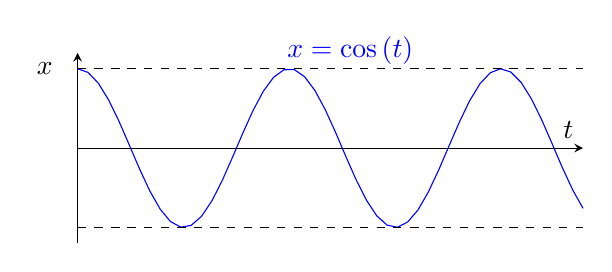
\begin{tikzpicture}
\begin{axis}[
        width = 8cm,
        height = 4cm,
        axis lines = middle,
        clip = false,
        xmin = 0,
        xmax = 5,
        ymin = -1.2,
        ymax = 1.2, 
        restrict y to domain=-1:2,
        ticks=none,
        xlabel = $t$,
        ylabel = $x$,
        y label style={at={(-0.1,1)}},
    ]

    \addplot+[mark=none,samples=50,unbounded coords=jump,domain=0:5 ]
    {cos(deg(3*x))}
    node [pos=0.4,above right]
    { $x=\cos\left(t\right)$};
    \addplot[dashed,mark=none,samples=50,domain=0:5 ] {1};
    \addplot[dashed,mark=none,samples=50,domain=0:5 ] {-1};
\end{axis}
\end{tikzpicture}
\end{center}

%%%%%%%%%%%%%%%%%%%%%%%%%%%%%%%%%%%%%%%%%%%%%
\subsubsection{Erzwungene Schwingung}
Erzwungene Schwingung bedeutet:
\begin{outline}
    \1 Schwach gedämpftes System ($\delta^2<\omega^2_0$)
    \1 Periodische Anregung
\end{outline}
\begin{eqnarr}
    m \ddot{x}+r\dot{x}+k x&=& F_0\sin( \omega t)\\
    \ddot{x}+\underbrace{\frac{r}{m}}_{2\delta} \dot{x}
                  +\underbrace{\frac{k}{m}}_{\omega_0^2} x
                  &=& \underbrace{\frac{F_0}{m}}_{k_0}\sin( \omega t)\\
\end{eqnarr}

Lösung:
\begin{eqnarr}
x(t) &=&  x_h+x_p \\
&=& e^{-\delta t}\left(
    C_1\sin\left( \omega_d t \right)+C_2\cos\left( \omega_d t \right)
\right)
    +A \sin\left( \omega t-\varphi \right)
\end{eqnarr}

Was passiert wenn $t\rightarrow \infty$?
\begin{equation*}
    x(t) = \underbrace{e^{-\delta t}\left(
        C_1\sin\left( \omega_d t \right)+C_2\cos\left( \omega_d t \right)
\right)
    }_{\rightarrow 0}
    +A \sin\left( \omega t-\varphi \right)
\end{equation*}

Die stationäre Lösung ist 
\begin{equation*}
    \boxed{x_p = A \sin(\omega t - \varphi)}
\end{equation*}

\begin{outline}
    \1[] $A=A(\omega)$: \underline{Amplitudengang}
    \1[] $\varphi=\varphi(\omega)$: \underline{Phasengang}
\end{outline}

Bestimmen von $A$ und $\varphi$: Komplex rechnen mit 
\begin{eqnarr}
    \underline{K}(t) &=& K_0 e^{j\omega t}\\
    \underline{x}(t) &=& A e^{j(\omega t-\varphi)}\\
    \Rightarrow &&\\
    K(t) &=& \text{Im }\underline{K}(t)\\
    x_p(t) &=& \text{Im }\underline{x}(t)\\
\end{eqnarr}
In DGL einsetzen
\begin{eqnarr}
    \underline{x}(t) &=& A e^{j(\omega t-\varphi)}\\
    \dot{\underline{x}}(t) &=& j\omega A e^{j(\omega t-\varphi)}\\
    \ddot{\underline{x}}(t) &=& -\omega ^2 A e^{j(\omega t-\varphi)}\\
\end{eqnarr}

\begin{eqnarr}
    -\omega ^2 A e^{j(\omega t-\varphi)}
    +2\delta j\omega A e^{j(\omega t-\varphi)}
    +\omega_0^2 A e^{j(\omega t-\varphi)} 
    &=& K_0 e^{j\omega t}\\
    -\omega ^2 A 
    +2\delta j\omega A
    +\omega_0^2 A 
    &=& K_0 e^{-j(\omega t-\varphi)} e^{j\omega t}\\
    -\omega^2A +2\delta j\omega A +\omega_0^2 A  &=& K_0  e^{j\varphi}\\
    \omega_0^2 -\omega^2 +j (2\delta \omega) 
        &=& \frac{K_0}{A}  e^{j\varphi}\\
\end{eqnarr}
\begin{center}
    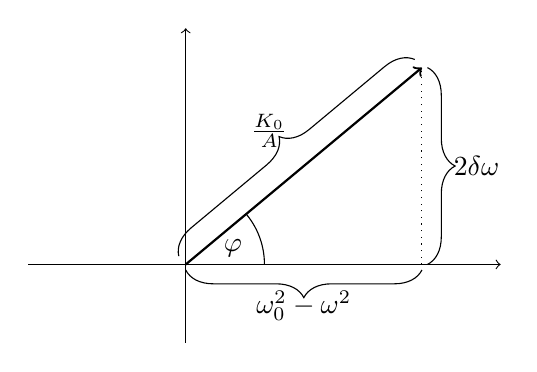
\begin{tikzpicture}
        \draw (-2,0) -- (0,0) -- (0,-1);
        \draw[<->] (0,3) -- (0,0) -- (4,0);

        \draw[->,thick] (0,0) -- (3,2.5);
        \draw[decorate,decoration={brace,amplitude=10pt},yshift=3pt,xshift=-2.5pt]
        (0,0) -- (3,2.5) node [midway,above left] {$\frac{K_0}{A}$};
        \draw[decorate,decoration={brace,mirror,amplitude=10pt},yshift=-2pt]
        (0,0) -- (3,0) node [midway,below,yshift=-4pt] {$\omega_0^2-\omega^2$};
        \draw[decorate,decoration={brace,mirror,amplitude=10pt},xshift=2pt]
        (3,0) -- (3,2.5) node [midway,right,xshift=6pt] {$2\delta\omega$};
        \draw[dotted] (3,0) -- (3,2.5) ;
        \node at (0.6,0.2) {$\varphi$};
        \clip (0,0) -- (3,0) -- (3,2.5) -- (0,0);
        \draw (0,0) circle[radius =1];
    \end{tikzpicture}
\end{center}
Pythagoras
\begin{equation*}
    \frac{K_0^2}{A^2} = \left( \omega_0^2 -\omega^2 \right)^2+4\delta^2\omega^2
\end{equation*}
$\Rightarrow$
\begin{equation*}
    \boxed{
        A = \frac{K_0}
        {\sqrt{\left( \omega_0^2-\omega^2 \right)^2+4\delta^2\omega^2}}
    }
\end{equation*}
Phase:
\begin{equation*}
    \tan\varphi = \frac{2\delta\omega}{\omega_0^2-\omega^2}
\end{equation*}
\begin{equation*}
    \boxed{
        \phi = \phi(\omega) = \left\{
            \begin{array}{lc}
            \arctan\left( \frac{2\delta\omega}{\omega_0^2-\omega^2} \right)
                & \omega<\omega_0 \\
            \frac{\pi}{2} & \omega=\omega_0\\
            \arctan\left( \frac{2\delta\omega}{\omega_0^2-\omega^2}\right)+\pi
                & \omega>\omega_0 \\
            \end{array}
        \right.
    }
\end{equation*}

\subsubsection*{Amplitudengang}
\begin{center}
\begin{tikzpicture}
\begin{axis}[
        width = \linewidth,
        height = 7cm,
        axis lines = middle,
        clip = false,
        xmin = 0,
        ymin = 0,
        ymax = 0.2, 
        restrict y to domain=0:0.2,
        ticks=none,
        xlabel = $\omega$,
        ylabel = $A$,
    ]

    \newcommand\OMEGA{3.8}

    \pgfmathdeclarefunction{A}{2}{%
        \pgfmathparse{%
            1 / sqrt( (\OMEGA^2-#1^2)^2 + 4*#2^2*#1^2 )%
        }%
    }
    \pgfmathdeclarefunction{wr}{1}{%
        \pgfmathparse{%
            sqrt(\OMEGA^2-2*#1^2)
        }%
    }

    \pgfplotsinvokeforeach {0,...,2} {
        \addplot+[mark=none,samples=50,unbounded coords=jump,domain=0:7 ] (
           {x},
           {A(x,#1)}
        )
        [yshift=8pt]
        node [pos=0.57,right] { $\delta = #1$ }
        ;
        \coordinate (omegaR#1) at (axis cs:{wr(#1)},0);
    }
    
    \draw[dotted] (omegaR0) node[below] {$\omega_0$} -- ++ (axis cs:0, 0.2);
    \draw[dotted] (omegaR1) node[below] {$\underset{\delta=1}{\omega_r}$} 
        -- ++ (axis cs:0, {A(wr(1),1});
    \draw[dotted] (omegaR2) node[below] {$\underset{\delta=2}{\omega_r}$} 
        -- ++ (axis cs:0, {A(wr(2),2});
    
\end{axis}
\end{tikzpicture}
\end{center}
\subsubsection*{Phasengang}
\begin{center}
\begin{tikzpicture}
    \begin{axis}[
            width = \linewidth,
            height = 7cm,
            axis lines = middle,
            clip = false,
            %xmin = 0,
            %ymin = 0,
            ymax = 1.2*pi, 
            %restrict y to domain=0:pi,
            ticks=none,
            xlabel = $\omega$,
            ylabel = $\varphi$, 
            use fpu=false,
    ]

        \newcommand\DELTA{0.2}
    
        \pgfmathdeclarefunction{phiF}{2}{%
            \pgfmathparse{%
                %rad(atan2(2*x, (#1^2-x^2)))
                rad(atan2((#2^2-x^2),2*#1*x )) % Wieso Argumente gedreht..??
            }%
        }

        \pgfplotsinvokeforeach {0.01,0.3,0.8} {
            \addplot+[mark=none,samples=100,domain=0:2] {phiF(#1,1)} 
            node[pos=0.7,below] {$\delta=#1$};
        }
    
        \draw[dotted] (axis cs:1,0) node[below] {$\omega_0$} 
        -- (axis cs:1,pi/2) -- (axis cs:0,pi/2) node[left] {$\frac{\pi}{2}$};
        \draw[dotted] (axis cs:0,pi) node[left] {$\pi$} -- (axis cs:2,pi);
    \end{axis}
\end{tikzpicture}
\end{center}

\subsubsection*{Berechnung von $\omega_r$}
$A(\omega)$ hat Maximum bei $w_r$, also gilt 
$\left.\frac{\partial}{\partial\omega} A(\omega)\right|_{\omega=\omega_r}=0$
    \begin{equation*}
        A(\omega) = \frac{K_0}
        {\sqrt{\left( \omega_0^2-\omega^2 \right)^2 + 4\delta^2\omega^2}}
    \end{equation*}
Wenn $A(\omega)$ Maximum hat, dann auch $A^2(\omega)$.\\
Wenn $A^2(\omega)$ Maximum hat, dann hat $\frac{1}{A^2(\omega)}$ ein Minimum.\\
Löse also 
\begin{eqnarr}
    0 &=& \left.\frac{\partial}{\partial\omega}
        \frac{1}{A^2(\omega)}\right|_{\omega=\omega_r} \\
        &=& \left.\frac{\partial}{\partial\omega} 
        \frac{\left( \omega_0^2-\omega^2
        \right)^2+4\delta^2\omega^2}{K_0^2}\right|_{\omega=\omega_r} \\
      &=& \frac{1}{K_0^2}\left( 
        2\left(\omega_0^2-\omega_r^2\right)\left(-2\omega_r\right)+8\delta^2
        \omega_r \right)\\
    0 &=& 4\omega_r \left( \omega_r^2 - \omega_0^2 + 2 \delta^2 \right) \\
    0 &=& \omega_r^2 - \omega_0^2 + 2 \delta^2 \\
    \omega_r &=& \sqrt{\omega_0^2-2\delta^2}
\end{eqnarr}

\begin{center}
    \begin{tabular}{lcc}
        \toprule
        \multicolumn{3}{c}{\textbf{Begriffe}}\\
        \midrule
        Name & Symbol & Formel \\
        \midrule
        Kreisfrequenz des ungedämpften Systems & $\omega_0$ & \\ \addlinespace
        Kreisfrequenz des gedämpften Systems & $\omega_d$ &
        $\sqrt{\omega_0^2-\delta^2}$ \\ \addlinespace
        Kreisresonanzfrequenz & $\omega_r$ & $\sqrt{\omega_0^2-2\delta^2}$
        \\\addlinespace
        Frequenz & $f$ & $\frac{\omega}{2\pi}$ \\\addlinespace
        Periodendauer & $T$ & $\frac{1}{f}$ \\\addlinespace
        \bottomrule
    \end{tabular}
\end{center}
